\documentclass[UTF8]{ctexart}
\usepackage{indentfirst}
\usepackage{apacite}
\usepackage{graphicx}
\bibliographystyle{apacite}

\title{比较不同排序算法的效率}
\author{张子健, 王颜睿, 梁铭恩, 陈亮沛, 戴益翔 \\ 佛山市第一中学}

\begin{document}
\maketitle
\begin{abstract}
	计算机科学中,时间复杂度往往被用于衡量排序算法的执行效率。但是在工程问题中,时间复杂度所忽略的低阶项以及常数因子往往成为限制实践的重要因素。在这篇论文中,我们分别编写六种常见比较排序(冒泡排序、选择排序、插入排序、堆排序、快速排序、归并排序)的实现并比较它们的运行效率。为了排除计算机体系架构和编译模式的影响,我们不计算程序运行时间,而是统计算法运行过程中发生的元素比较和元素赋值的次数。
\end{abstract}

\section{引言}

\section{相关工作}

\paragraph{时间复杂度}
在计算机科学中,时间复杂度 \cite{cormen1990introduction} 往往被用于衡量一个算法的执行效率。这是一个代表算法输入值的字符串的长度的函数。时间复杂度常用大$O$符号表述,不包括这个函数的低阶项和首项系数。使用这种方式时,时间复杂度可被称为是渐近的,亦即考察输入值大小趋近无穷时的情况。解决同一个问题,时间复杂度越低,该算法效率越高。算法的时间复杂度忽略了所有的低阶项和常数时间,因此只能定性描述算法的运行效率。但是,在工程问题中,算法的常数时间往往对最终的效果有明显的影响。因此,横向对比不同排序算法的实际运行效率很有必要。

\paragraph{堆排序}
堆排序\cite{cormen1990introduction}是指利用堆积树(堆)这种数据结构所设计的一种排序算法,它是选择排序的一种。可以利用数组的特点快速定位指定索引的元素。堆分为大根堆和小根堆,是完全二叉树。对于一个大小为$n$的无序序列,每一次读入的元素$a_i$,都会被插入到堆中,维护堆需要$\log i$次操作。读入$n$次,需要做$\sum_{i=1}^{n}\log i$次。在输出结果时,第i次直接输出堆顶的元素(最大或最小),然后删除堆顶并维护堆,需要做$\log (n-i)$次操作。输出n次,需要做$\sum_{i=1}^{n}\log i$次。综上,整个排序过程,一共要做$2\sum_{i=1}^{n}\log i$次操作,所以堆排序的时间复杂度为$O(n \log n)$的数量级。

\paragraph{归并排序}
归并排序\cite{cormen1990introduction}是建立在归并操作上的一种有效的排序算法,该算法是采用分治法的一个非常典型的应用。将已有序的子序列合并,得到完全有序的序列;即先使每个子序列有序,再使子序列段间有序。若将两个有序表合并成一个有序表,称为二路归并。归并排序是一种稳定的排序方法。对于读入和输出一个大小为n的无序序列,各需要n次操作。排序时,需要运用递归,先排好当前序列。对于已经排好序的两个子序列,将两个序列各自第一个元素中更小或更大的(如果相同,则选择)加入辅助数组,然后后移操作过的序列的指针,直到两个序列都为空。由于每个子序列中的第一个元素必定是该序列的最值,则两个子序列中各自第一个元素的最值必然是整个序列的最值,就能保证辅助数组的有序性,所以该步骤的正确性是有保证的。由于每次这个步骤需要n次操作,根据二分法需要分$\log n$次,所以需要$n \log n$此操作。加上输入和输出,该算法的复杂度为$O(\log n)$。

\paragraph{冒泡排序}
冒泡算法\cite{cormen1990introduction}的基本思想是依次把最大(最小) 数浮动到正确位置。冒泡算法对数据进行N次迭代,每次迭代都按顺序比较序列的连续两个元素并把较大数往后移动,从而实现每次迭代将一个未排好的最大值排到正确位置,在N次后必然排好序列。由于进行n次迭代,每次迭代遍历一次序列,故时间复杂度为$O(N^2)$。而空间除原数据外没有与N有关的额外存储,故空间复杂度为$O(1)$。

\paragraph{插入排序}
插入算法的基本思想是在已排序好的序列里插入未排序的元素(如打扑克时人们常用的排序)。插入排序\cite{cormen1990introduction}要进行n次迭代,每次迭代将一个无序元素插入到有序序列,进行n次后所有无序元素均插入到有序序列,排序完成。由于进行了n次迭代,因此时间复杂度关键取决于插入操作。显然,最好情况是有序序列,插入过程只需比较一次,时间复杂度为 $O(N)$ ;最坏情况是倒序序列,插入过程平均比较 $n \over 2$ 次,时间复杂度为 $O(\frac{n^2}{2})$与冒泡排序相同,插入排序没有使用额外空间,空间复杂度为 $O(1)$

\paragraph{快速排序}
快速排序是一种不稳定的排序算法,简称快排,由英国计算机科学家查尔斯·安东尼·理查德·霍尔爵士提出。他的操作流程为:

\begin{itemize}
	\item 每次选定一个基准值
	\item 把当前区间内的数根据这个基准值分为两个区间,其中一区间大于这个基准值,另一区间小于这个基准值
	\item 只要某一个区间内有数,就进行①②操作,直到分出来的这个两区间为空才终止程序
\end{itemize}

根据以上过程可以推断出它在最有情况下和最劣情况下的时间复杂度:
\subparagraph{最优情况}
我们每次选定的基准点恰好为位于当前整个区间的中位数,即刚好把整个区间对称分开,例如当前区间内有$n$个数,选定的基准点为区间的中位数,以中位数为基准点划分后,一个区间内的数为$(n-1)/2$(向下取整)个数,另一个区间内的数即为$n - 1 - (n-1) \over 2$个数,那么我们每次都可以大概的看为对半划分,假设数据范围为n,那么我们递归的层数为$log2^n$,每层的时间复杂度为$O(n)$,所以最优情况下总的复杂度为:递归的层数*每层的时间复杂度$O(log2^n)*O(n)=(O(nlog2^n)$

\subparagraph{最劣情况}
设当前区间的大小为$n$时,当选定的基准点为这个区间的最值的时候,只能把区间分为一个空区间和一个有$(n-1)$个数的区间,那么我们每次递归了一层,待操作的数就会减一,那么第k层待比较的个数为$(n-k+1)$,有$n$层,总的时间复杂度为$O(n*(1+2+3+...+n))=O(n*(n+1)*n/2)=O(n^(2))$。为了尽可能避免最劣情况的出现,我们可以取当前区间的头、尾、中间数三个数之间的中位数来用作基准点,来减少最不理想情况下的用时。

\subparagraph{期望情况}
作为递归算法,快速排序的平均复杂度可以写:$O(n)=n-1+\frac{1}{n}\sum_{i=1}^{n-1}(O(n-1-i)+O(i))=O(2n\ln{n})≈O(1.39 n \log_2 n)$。在做题以及实际应用时,快速排序通常被认为是$O(nlog{n})$的算法

快速排序根据写法的不同可以也分为原地排序和非原地排序两种,两种写法的空间复杂度也不一样。快速排序本来的时间复杂度是O(n)的,主要产生的空间复杂度是由于递归调用。由于情况比较多,以及在不同定义下描述的空间复杂度都有所出入,并且在实际使用中空间复杂度对快速排序的约束不大,限于编者能力,这里不加以详细讨论。

\section{方法}
我们根据\citeauthor{cormen1990introduction}的伪代码分别编写六种常见比较排序(冒泡排序、选择排序、插入排序、堆排序、快速排序、归并排序)的测试程序,追踪每一次定义在源程序代码中的元素比较和变量赋值并统计最终结果。我们采用同一个程序,仅改变用于排序的函数以得到结果,并最大限度避免因为人为程序编写误差导致的结果偏差。

\paragraph{样本生成}
对于每个排序算法,我们选择数据规模 $2^7$、$2^8$、$2^9$······$2^{19}$、$2^{20}$ 各20组(部分时间复杂度为$O(n^2)$的排序算法由于计算量过大不能取到$2^{20}$ 数据规模)。对于每个数据规模,我们生成了20组互不相同的,值范围为  $[0, 1)$ 的数据。

\section{实验}
我们在配备英特尔\textregistered 酷睿\texttrademark i3-6100处理器、4GB DDR3-1600MHz内存以及Ubuntu 18.04 LTS与GNU C++ Compiler 4.8.5的计算机上运行我们的样例程序。

\begin{figure}[h]
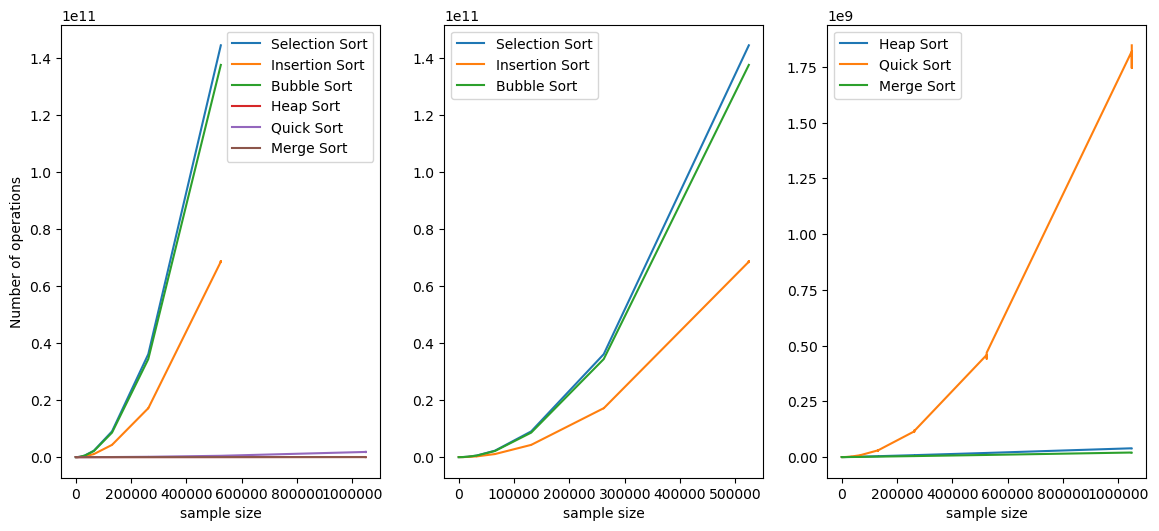
\includegraphics[width=\textwidth]{fig1.png}
\caption{六种排序算法的比较}
\end{figure}

\section{结语}

\renewcommand{\refname}{参考文献}
\bibliography{article}
\end{document}
